
\chapter{Обобщение полученных результатов}

Исследуя модельный порыв, удалось получить некоторое представление о его внутренней структуре и механизме поддержания колебаний в нем. В настоящей главе поднимается вопрос о том, какое отношение выделенные механизмы имеют к организации движения жидкости в других режимах течения. В настоящее время известно достаточно большое число решений уравнений Навье-Стокса в виде бегущих волн и условно периодических решений  \cite{Kawahara2012}. Примером условно периодического решения является модельный порыв --- его поле скорости меняется периодическим образом в подходящей подвижной системе отсчета. Простота временного поведения таких решений позволяет выполнить их детальное исследование. Полученные результаты дают возможность оценить универсальность выделенных при исследовании модельного порыва механизмов. 

Продолжая модельный порыв по числу Рейнольдса в работе удалось найти новые условно периодические по времени решения. В частности, найдены условно периодические решения, по скорости сноса и амплитуде колебаний оказывающиеся ближе к турбулентному порыву, чем исходное решение. Также в работе получено несколько семейств решений, имеющих вид бегущих волн, в течении Гагена-Пуазейля и в плоском течении Пуазейля. Описаны основные свойства найденных решений и механизм поддержания колебаний в них. Все решения воспроизводят идентичный механизм поддержания колебаний, согласующийся с механизмом, выделенным в модельном порыве, что говорит о некоторой универсальности этого механизма. В главе приведено описание метода Ньютона-Крылова, позволяющего находить условно периодические решения уравнений Навье-Стокса, а также решения, имеющие вид бегущей волны, как частный случай условно периодических решений. Дано описание метода продолжения по параметру, опирающегося на метод Ньютона-Крылова для поиска условно периодических решений. Приведен анализ найденных решений. Анализ решений в виде бегущей волны, найденных в плоском течении Пуазейля, опубликован в работах автора \cite{Vest18, KMU16}. 

\section{Метод Ньютона-Крылова для поиска условно периодических решений уравнений Навье-Стокса}

Условно периодическим мы называем решение уравнений Навье-Стокса, являющееся периодическим по времени в подходящей подвижной системе отсчета. В работе реализован метод Ньютона-Крылова \cite{Sanchez2004}, позволяющий численно находить условно периодические решения. Поле скорости $\v_p(x,r,\theta)$ соответствует условно периодическому решению, если интегрирование уравнений движения c $\v_p$ в качестве начального поля скорости в течении времени $T_p$ в системе отсчета, перемещающейся со скоростью $c_p$, дает поле скорости, совпадающее с $\v_p$:
\begin{equation}\label{P_eq}
\phi(\v_p, T_p, c_p, \Re) = \v_p.
\end{equation}
В этом случае $T_p$  --- временной период решения. Функция $\phi(\v, t, c, \Re)$ имеет значение поля скорости, полученного интегрированием уравнений движения при начальном поле скорости $\v$ в течении времени $t$ в системе отсчета, перемещающейся со скоростью $c$, при числе Рейнольдса $\Re$. Заметим, что при условии несжимаемости давление в каждый момент времени с точностью до константы определяется мгновенным полем скорости, что позволяет исключить давление из \eqref{P_eq} и других уравнений. 

Если $\v_1(x,r,\theta)$ --- решение \eqref{P_eq}, то $\v_2(x, r, \theta) = \v_1(x + \Delta x, r, \theta)$ и $\v_3 = \phi(\v_1, \Delta t, c, \Re)$ при произвольных $\Delta x$ и $\Delta t$ также являются решениями \eqref{P_eq}, соответствующими одному условно периодическому решению уравнений Навье-Стокса. Для того, чтобы с каждым условно периодическим решением связать только одно поле скорости $\v_p$, на решения уравнения \eqref{P_eq} накладываются два дополнительных условия. Условия могут быть выбраны, например, таким образом, чтобы полю скорости $\v_p$ соответсвовал момент времени, в который амплитуда пульсаций в течении достигает наибольшей амплитуды, и наибольшее отклонение от течения Пуазейля достигается в центре расчетной области. 

Нелинейное уравнение \eqref{P_eq} с двумя дополнительными условиями решается численно методом Ньютона. Метод Ньютона итерационный и на каждом шаге позволяет уточнить существующее приближение к решению. Для системы $F(x) = 0$ метод Ньютона формулируется следующим образом. Пусть $x_m$ --- приближение к решению на шаге $m$, $x^*$ --- точное решение. Разложение $F(x^*)$ в ряд около точки $x_m$ имеет вид:
\begin{equation}
F(x^*) = F(x_m) + \pd{F}{x}\bigg|_{x=x_m} \Delta x_m^* + O(\Delta x_m^{*2}), 
\end{equation}
где $\Delta x_m^* = x^* - x_m$. Пренебрегая нелинейными относительно $\Delta x_m^*$ слагаемыми, учитывая, что $F(x^*) = 0$, получим линейную систему на поправку к решению:
\begin{equation}\label{Newton_eq}
J \Delta x_m = b,
\end{equation}
где $J$ --- матрица Якоби:
$$
J = \frac{\partial F}{\partial x}\bigg|_{x = x_m},
$$
вектор $b = - F(x_m)$. 
Основной задачей при применении метода Ньютона является решение линейной системы \eqref{Newton_eq}. Новое приближение к решению вычисляется по формуле: 
\begin{equation} \label{end_NK_eq}
x_{m+1} = x_m + \Delta x_m. 
\end{equation}

Для решения линейной системы \eqref{Newton_eq} применяется итерационный алгоритм, в котором приближение к решению находится в подпространствах Крылова $K_i = span\{b, Jb, J^2b, ... , J^ib\}$, где $span\{a_1, ..., a_i\}$ обозначает линейную оболочку векторов $a_1, ..., a_i$. Построение базиса в подпространстве $K_{i+1}$ при условии, что базис в подпространстве $K_i$ уже известен, требует одного умножение уже известного вектора $J^ib$ на $J$ ($K_0 = span\{b\}$). Произведение матрицы Якоби $J$ на вектор единичной длины $e$ равно производной от функции $F$ в соответствующем направлении:
\begin{equation} \label{Je_eq}
Je = \pd{F}{x} e = \pd{F}{e}. 
\end{equation}
Таким образом, построение базиса в подпространствах Крылова сводится к вычислению производных по направлению от функции $F$. Значение производной функции $F$ по направлению $e$ приближается конечной разностью, которая может быть найдена численно:
\begin{equation}\label{fd_eq}
\pd{F}{e} \approx \frac{F(x + \varepsilon e) - F(x)}{\varepsilon}.
\end{equation}
В наших расчетах действительные числа представляются 64-битными числами с плавающей запятой. В этом случае значение $\varepsilon$ рекомендуется выбирать близким к $10^{-7}$ \cite{Viswanath2007}. Метод Ньютона, в котором приближения к решениям системы \eqref{Newton_eq} находятся в подпространствах Крылова, называют также методом Ньютона-Крылова \cite{Sanchez2004}. 

В работе для решения линейной системы \eqref{Newton_eq} применяется метод минимизации невязки \cite{EEbook}. Этот метод также итерационный. На $i$-ом шаге выполнения метода в подпространстве Крылова $K_i$ ищется приближение к решению $x_i$ таким образом, что невязка $r_i = b - Ax_i$ имеет наименьшую длину. Критерием остановки итерационного процесса служить снижение длины невязки ниже заранее заданной величины, либо превышение заранее заданного числа итераций. При поиске условно периодических решений с небольшим числом неустойчивых направлений (менее 10), для уточнения решения на порядок требуется несколько десятков итераций метода минимизации невязки, причем число итераций  практически не зависит от параметров расчетной сетки (при условии, что сетка достаточно подробна для адекватного воспроизведения решения) \cite{Dijkstra2014}. На каждой итерации метода минимизации невязки требуется однократно вычислить значение функции $F$ в новой точке. В нашем случае вычисление функции $F$ связано с численным интегрированием уравнений движения в течении времени $T_p$, что требует значительных вычислительных ресурсов. Сравнительно небольшое число обращений к функции $F$ делает реализованный метод Ньютона-Крылова эффективным инструментом поиска условно периодических решений, имеющих небольшое число неустойчивых направлений.

Для построения подпространств Крылова необходимо, чтобы матрица $J$ была квадратной. Если поле скорости задается $N$ параметрами, то в матрице $N+2$ строки. Соответственно, вместе с полем скорости в число неизвестных необходимо включить два параметра системы, например, временной период $T_p$ и скорость системы отсчета $c_p$. Тогда свободным параметром остается только число Рейнольдса $\Re$, $T_p$ и $c_p$ играют роль собственных значений системы, при которых условно периодическое решение существует. 

Критерием остановки итерационного процесса метода Ньютона может служить снижение нормы невязки ниже заранее заданной величины, либо превышение заранее заданного числа итераций. 


%Невязка имеет наименьшую длину, если она перпендикулярна пространству $AK_i$. Проще всего опустить перпендикуляр из вектора $b$ на подпространство $AK_i$, имея в этом подпространстве ортогональный базис. Построим последовательность векторов $q_1, \dots, q_i$ таким образом, что они образуют базис в подпространстве $K_i$, а вектора $p_1 = Aq_1, \dots, p_i = Aq_i$ образуют ортогональный базис в подпространстве $AK_i$. Тогда легко может быть построено ортоганальное разложение правой части уравнения вида $b = \alpha_1 p_1 + \dots + \alpha_i p_i + r_i$, где $b_i =  \alpha_1 p_1 + \dots + \alpha_i p_i$ лежит в пространстве $AK_i$, а $r_i$ перпендикулярно ему. Коэффициенты разложения дает формула:
%\begin{equation}
%\alpha_k = (b,p_k) / (p_k, p_k),
%\end{equation}
%где $(\ ,\ )$ ---  скалярное произведение, порождающее норму, в которой минимизируется невязка. 
%Так как у каждого вектора $p_k$ известен прообраз $q_k$, линейная комбинация векторов $q_k$ с коэффициентами $\alpha_k$ дает приближение к решению, лежащее в пространстве $K_i$
%\begin{equation}
%\x_i = \alpha_1 q_i + \dots + \alpha_i q_i. 
%\end{equation}
%Переход на $i+1$ итерацию алгоритма связан с построением базиса подпространств $K_{i+1}$ и $AK_{i+1}$. Для построения ортогонального базиса в подпространстве $AK_{i+1}$ базис подпространства $AK_i$ пополняется новым вектором $p_{i+1}$, полученным ортогонализацией с уже известными базисными векторами $p_1, \dots, p_i$ вектора $Ap_i$. В процессе ортогонализации также может быть получен вектор $q_{i+1}$, являющийся прообразом вектора $p_{i+1}$. 

%Критерием остановки итерационного процесса при решении линейной системы может служить снижение величины невязки ниже заранее заданного порогового значения, либо превышение заранее заданного числа итераций. Переход на новый шаг выполнения метода требует однократного вычисления произведения матрицы $A$ на вектор, связанного с вычисление производной функции $F$ вдоль одного направления в соответствии с \eqref{Jl_eq}, \eqref{fd_eq}. В процессе вычислений необходимо хранить две последовательности векторов $p_1, \dots, p_i$ и $q_1, \dots, q_i$. На первой итерации $q_1 = b$, $p_1 = Ab$.  


\section{Продолжение модельного порыва по числу Рейнольдса} \label{contin_sec}

Основной сложностью при нахождении новых условно периодических решений оказывается подбор подходящего начального приближения к решению, с которым метод Ньютона сойдется. Однако если одно условно периодическое решение известно, оно может быть использовано в качестве начального приближения для решения с близкими значениями параметров. Найденное решение, в свою очередь, также может выступать в качестве начального приближения к новому решению при новом значении параметров. Таким образом, может быть построена цепочка решений, связывающая решения с различными значениями параметров. Говорят, что решение в этом случае продолжается по этим параметрам \cite{Viswanath2007, Dijkstra2014}. 

Продолжая решение, соответствующее модельному порыву, по числу Рейнольдса, удалось получить новые условно периодические решения с пространственно локализованной структурой. На рисунке \ref{local_contin_pic} представлены значения $T_p$, $c_p$ и $\Re$ для найденных таким образом решений. Как показывают расчеты, решения принадлежат однопараметрическому множеству, что согласуется с \cite{Avila2013}. Решения, принадлежащие различным кривым, найдены на различных расчетных сетках. Параметры сеток, на которых выполнены расчеты, приведены в разделе \ref{edge_seq}. Черная точка на каждом из графиков соответствует исходному решению --- модельному порыву. При $\Re = 1400$ обнаружена точка бифуркации, в которой порождаемое модельным порывом семейство решений рождается (в \cite{Avila2013} сообщается о $\Re^* = 1430$). При меньших значениях числа Рейнольдса решений не существует. При больших значениях числа Рейнольдса существует две ветви решений, то есть при каждом значении $\Re$ существует два решения, каждое из которых принадлежит свой ветви. Исходное решение принадлежит нижней ветви решения (на графиках она оказывается выше). Для решений с нижней ветви характерна меньшая амплитуда колебаний, меньшая интенсивность поперечного движения и большие значения $T_p$ и $c_p$. Для того, чтобы в точке бифуркации перейти с нижней ветви решений на верхнюю, можно включить $\Re$ в число определяемых параметров, а продолжение решения выполнить по $T_p$ или $c_p$. Для того, чтобы адекватно воспроизвести решения с верхней ветви, необходимы более подробные расчетные сетки. Характеристики решений с верхней ветви, полученные на различных сетках, согласуются между собой до $\Re \approx 1700$. При больших $\Re$ между решениями, полученными на различных сетках, начинают проявляться некоторые качественные отличия. Для более подробного анализа верхней ветви решений выбрано решение при $\Re = 1700$. Мы полагаем, что используемые нами расчетные сетки позволяют адекватно воспроизвести это решение. 


\begin{figure}
\center{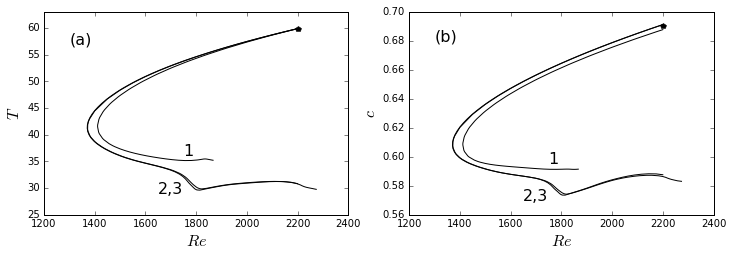
\includegraphics[width=0.9\linewidth]{local_contin.png}}
\caption{Продолжение решения, соответствующего модельному порыву, по числу Рейнольдса. Изображены зависимость периода изменения решения во времени $T$ и скорости его перемещения вдоль трубы $c$ от числа Рейнольдса $\Re$. Кривые 1, 2 и 3 соответствуют решениям, полученным на различных расчетных сетках. Черные точки соответствует исходному решению, принадлежащему сепаратрисе.}
\label{local_contin_pic}
\end{figure}

Решения с верхней ветви сохраняют пространственно локализованную структуру, но её скорость перемещения оказывается ниже, амплитуда колебаний и интенсивность поперечного движения оказываются выше 


однако они обладают меньшей скорость перемещения вдоль трубы и меньший период изменения во времени. Для них характерна б\'{о}льшая интенсивность пульсаций и вторичных структур. Параметры решения на верхней ветви приближаются к параметрам турбулентного порыва. Это повышает ценность выводов, полученных при изучении решения  с верхней ветви. 

%Если решения с нижней ветви находится на границе области притяжения турбулентного режима течения (на сепаратрисе), то решения с верхней ветви расположены внутри нее и могут участвовать в формировании турбулентного аттрактора\cite{Avila2013}. 

\begin{figure}
\center{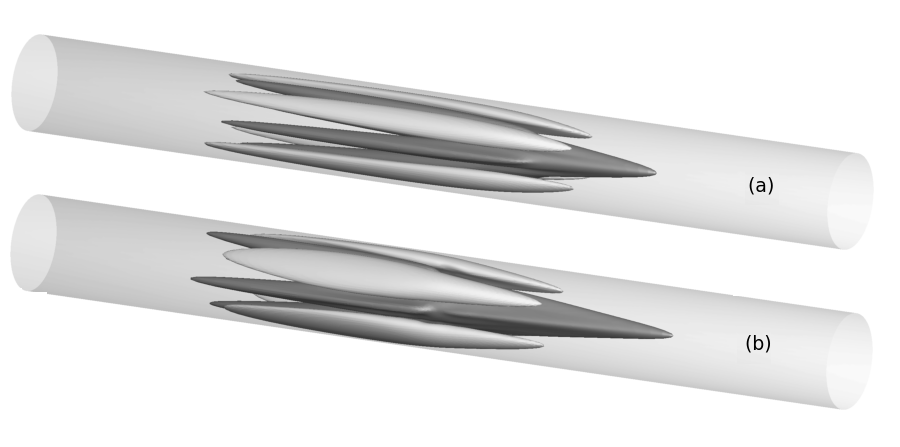
\includegraphics[width=0.9\linewidth]{3D_contin_cmp.png}}
\caption{Среднее поле скорости условно периодических решений, принадлежащих нижней (1) и верхней (2) ветви, при $\Re = 1700$ (2). Темным и светлым тоном выделены поверхности скорости $-0.1$ и $+0.1$ относительно скорости течения Пуазейля. Поток направлен слева направо.}
\label{3D_contin_cmp_pic}
\end{figure}

Среднее поле скорости выбранного для дальнейшего исследования решения представлено на рисунке \ref{3D_contin_cmp_pic} внизу. Для сравнения изображено также среднее поле скорости модельного порыва вверху. Качественно структура решения не меняется, однако интенсивность полос на верхней ветви выше, чем на нижней. Период по времени выделенного решения можно оценить в $T = 35$, скорость его перемещения вдоль трубы в $c = 0.59$ (скорость перемещения турбулентного порыва вдоль трубы близка к $0.5$). 



Продлевая решение, соответствующее модельному порыву, по числу Рейнольдса, удалось достичь точки бифуркации, в которой возникает две ветви решения, и перейти с нижней ветви на верхнюю. Как и модельный порыв, решение с верхней ветви локализовано в пространстве и является условно периодическим по времени, но его характеристики оказываются ближе к характеристикам турбулентного порыва. Параметры выбранного для исследования решение: $\Re = 1700$, $T = 35$, $c = 0.59$. Особенности, выделенные при изучении модельного порыва, могут быть в полной мере обобщены на решение с верхней ветви. 


\begin{figure}
\center{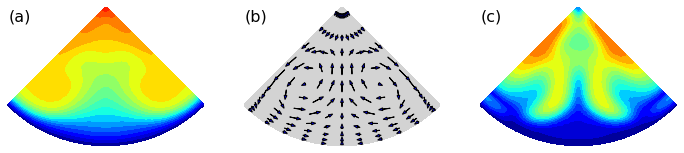
\includegraphics[width=0.9\linewidth]{local_ub_means.png}} 
\center{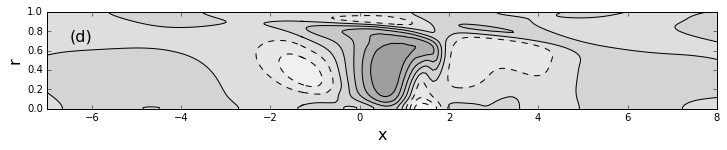
\includegraphics[width=0.9\linewidth]{local_ub_vel1.png}}
\caption{Поле скорости решения с верхней ветви. В сечении, где пульсации достигают наибольшей амплитуды, приведены: (a) --- $V_{x}$, (b) --- $(V_{r}, V_{\theta})$, (c) --- амплитуда $\v_n$; (d) --- мгновенное поле скорости $\v_n$ в сечении $\theta = 0$. }
\label{local_ub_means_pic}
\end{figure}


Как и в модельном порыве, в выделенном решении присутствуют полосы повышенной и пониженной скорости, вытянутые вдоль потока (смотри рисунок \ref{3D_contin_cmp_pic}). При разделении поля скорости решения $\v$ на среднюю $\V = \overline{\v}^t$ и пульсационную $\v_n = \v - \V$ составляющие, полосы попадают с среднюю составляющую движения. Продольная компонента среднего течения $V_x$ изображена на рисунке \ref{local_ub_means_pic}(a). Представлено только одно сечения, однако в других сечениях качественно картина не меняется. Полосы формируются за счет действия продольных вихрей, которые попадают в поперечную компоненту среднего течения $(V_r, V_\theta)$, в том же сечении представленную на рисунке \ref{local_ub_means_pic}(b). Пульсационная составляющая движения $\v_n$ имеет более сложную форму, чем в модельном порыв, однако в первую очередь она представляет собой бегущую вниз по потоку волну. Мгновенное поле скорости пульсационной составляющей движения $\v_n$ в продольном сечении $\theta = 0$ представлено на рисунке \ref{local_ub_means_pic}(d). На рисунке \ref{local_ub_means_pic}(с) представлена амплитуда пульсаций в том же сечении трубы. 


\begin{figure}
\center{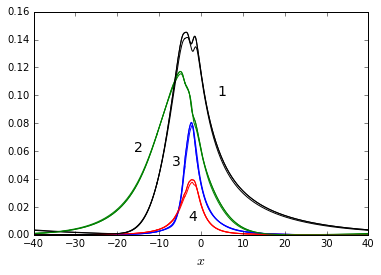
\includegraphics[width=0.6\linewidth]{amp_ub.png}}
\caption{Представлено распределение вдоль трубы амплитуды компонент движения решения с верхней ветви, $\Re = 1700$. Кривая 1 --- отклонение от течения Пуазейля поля скорости $V_{2D}$, кривые 2,3 --- продольная а поперечная компоненты поля скорости $\V_{3D}$, кривая 4 --- средняя по времени $\v_n$. Представлены результаты, полученных на трех расчетных сетках.}
\label{amp_ub_pic}
\end{figure}


На рисунке \ref{amp_ub_pic} изображена средняя по сечению трубы амплитуда различных компонент движения. Как при исследовании модельного порыва, среднее течение разделено на двумерную $\V_{2D} = \overline{\V}^{\theta}$ и трехмерную $\V_{3D} = \V - \V_{2D}$ составляющие. Полосы и продольные вихри попадают в трехмерную составляющую движения. Качественно, распределение интенсивности различных компонент двжиения вдоль трубы в выделенном решении и в модельном порыве совпадают (смотри рисунок \ref{amp_pic}), однако все компоненты движения в выделенном решении имеют большую амплитуду. Интенсивность полосчатого и пульсаций выше примерно в двое. Интенсивность продольных вихрей выше почти в четыре раза. На рисунке \ref{amp_ub_pic} представлены результаты, полученные на трех различных расчетных сетках, описанных в предыдущем разделе. Результаты, полученные на всех сетках, близки друг к другу, что подтверждает достаточность каждой из них для адекватного воспроизведения решения. 



Как в случае модельного порыва, в рассматриваемом случае среднее поле скорости решения на сепаратрисе оказывается линейно неустойчиво. Наиболее быстрорастущее возмущение, возникающее на среднем течении в рамках линеаризованных уравнений \eqref{lin_eq}, воспроизводит форму пульсационной составляющей движения. Оно может быть представлено в виде $\v'_1(x,r,\theta) e^{\lambda_1 t}$. Соответствующий инкремент нарастания оказывается равен $\lambda_1 = 0.014$. В силу относительной однородности среднего течения вдоль трубы, возникающее на нем возмущение близко к бегущей волне. Средняя по времени амплитуда возмущений $\v'_1$ представлена на рисунке \ref{ub_lin_pic}(a) в том же сечении, в котором пульсационная составляющая движения представлена на рисунке \ref{local_ub_means_pic}(c). Поле скорости $\v'_1$ в продольном сечении $\theta = 0$ представлена на рисунке \ref{ub_lin_pic}(b). В этом же сечении приведено мгновенное поле $\v_n$ на рисунке \ref{local_ub_means_pic}(d). Пульсации, возникающие в линейном приближении, $\v_1$, воспроизводят пульсационную составляющую движения $\v_n$, что говорит о том, что $\v_n$ возникает в следствии линейной неустойчивости среднего течения. Отметим, что поле скорости $(V_x, 0, 0)$ оказывается устойчиво к малым возмущениям, соответствующий инкремент затухания приблизительно равен $\lambda = -0.009$. 


\begin{figure}
\center{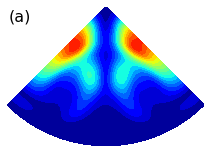
\includegraphics[width=0.3\linewidth]{ub_lin_cs.png} 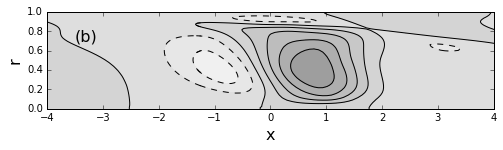
\includegraphics[width=0.6\linewidth]{ub_lin_ls.png}}
\caption{Наиболее быстрорастущее возмущение, возникающее на среднем течении в рамках линеаризованных уравнений \eqref{lin_eq}. Представлены: (a) --- амплитуда пульсаций в поперечном сечении трубы, как на рисунке \ref{local_ub_means_pic}(c); (b) --- мгновенное поле скорости в сечении $\theta = 0$, как на рисунке \ref{local_ub_means_pic}(d). }
\label{ub_lin_pic}
\end{figure}

Полосы повышенной и пониженной скорости возникают вследствие действия стационарных продольных вихрей. 
Механизм образования продольных вихрей в решении с верхней ветви и в модельном порыве также совпадают. На рисунке \ref{ub_OXgen_pic}(a) приведен квадрат средней продольной завихренности $\Omega_x^2$ в одном сечении трубы. Его распределение по сечению трубы соответствует паре продольных вихрей, расположенных между полосами повышенной и пониженной скорости. Определяющий вклад в образование $\Omega_x^2$ дают слагаемые \eqref{time_OXgen_terms}. Их вклад представлен на рисунке \ref{ub_OXgen_pic}(b). Вклад других слагаемых в правой части \eqref{time_OX_eq}, представленный на рисунке \ref{ub_OXgen_pic}(с), существенного влияния на форму продольных вихрей не оказывает. Также на рисунке \ref{ub_oxgen_lines_pic}(a) изображено распределение $\Omega_x^2$ и слагаемых, отвечающих за его формирование, на прямой, проходящей через область, занятую положительным вихрем. Он также подтверждает представления о том, что за образование продольных вихрей ответственно слагаемое \eqref{time_OXgen_terms}. Можно также отметить, что кривые 2 и 3 на рисунке \ref{ub_oxgen_lines_pic}(a) повторяют многие особенности друг друга, но с разным знаком, так что при сложении эти особенности пропадут. Это может быть связано с тем, что слагаемые \eqref{time_OXgen_terms} в этом случае не очень точно соответствуют слагаемым, представляющим физический механизм, ответственный за образование продольных вихрей. 
 

\begin{figure}
\center{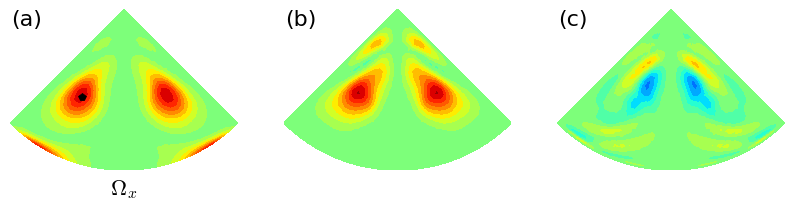
\includegraphics[width=0.9\linewidth]{ub_OXgen_map.png}}
\caption{Для решения с верхней ветви в сечении, где амплитуда пульсаций достигает наибольшего значения, представлены: (a) --- $\Omega_x^2$, (b) и (c) --- вклад в формирование $\Omega_x^2$ со стороны слагаемых \eqref{time_OXgen_terms} и суммы других слагаемых в правой части \eqref{time_OX_eq}. Черная точка на рисунке (a) соответствует прямой, значения на которой представлены на рисунке \ref{ub_oxgen_lines_pic}. Ноль по оси $x$ расположен в сечении, где амплитуда пульсаций достигает максимума.}
\label{ub_OXgen_pic}
\end{figure}

Механизм образования пульсационной составляющей продольной завихренности также сохраняется. На рисунке \ref{ub_oxgen_lines_pic}(b) также, как на рисунке (a), приведено значение амплитуды пульсационной составляющей движения $\overline{\omega'_x\omega'_x}^t$ и вклад в её образование со стороны различных слагаемых в уравнении \eqref{time_ox1_eq}. В области существования продольных вихрей определяющий вклад в образование пульсаций продольной завихренности дает слагаемое \eqref{time_ox1gen_term2}. Его вклад в $\overline{\omega'_x\omega'_x}^t$ изображен кривой 3. Другие слагаемые в правой части \eqref{time_ox1_eq} дают значительно меньший вклад. В частности, слагаемое \eqref{time_ox1gen_terms1}, ответственное за поворот нормальных к стенке вихрей, возникающих в пульсационной составляющей движения, в выделенной области близко к нулю. В этом случае также можно отметить неточность разделения на слагаемых в правой части \eqref{time_ox1_eq} на связанные и несвязанные в механизмом образования пульсаций $\omega'_x$, так как кривые 3 и 4 имеют ряд особенностей, пропадающих при сложении.

\begin{figure}
\center{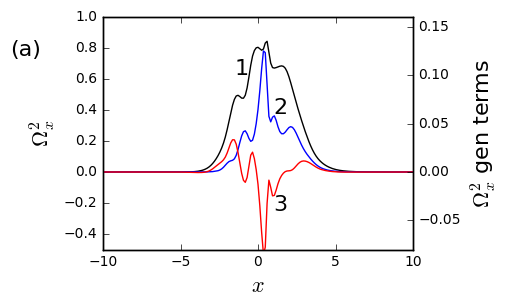
\includegraphics[width=0.5\linewidth]{ub_OXgen_lines.png}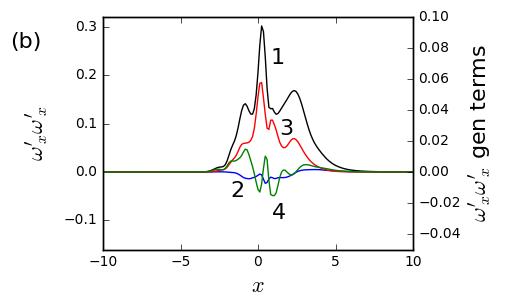
\includegraphics[width=0.5\linewidth]{ub_ox1gen_lines.png}}
\caption{Для решения с верхней ветви на прямой, проходящей через область, занятую положительным вихрем, при $r = 0.6$, $\theta = \pi/10$, представлены: график (a) --- $\Omega_x^2$ (кривая 1) и вклад в его формирование со стороны слагаемых \eqref{time_OXgen_terms} (кривая 2) и других слагаемых в правой части \eqref{time_OX_eq} (кривая 3); график (b) --- $\overline{\omega'_x\omega'_x}^t$ (кривая 1) и вклад в её формирование со стороны слагаемых \eqref{time_ox1gen_terms1} (кривая 2), слагаемого \eqref{time_ox1gen_term2} (кривая 3) и других слагаемых в правой части уравнения \eqref{time_ox1_eq} (кривая~4). Выделенной прямой соответствует черная точка на рисунке \ref{ub_OXgen_pic}(a). Соответствующий рисунок для модельного порыва --- \ref{xline_oxgen_pic}.} 
\label{ub_oxgen_lines_pic}
\end{figure}

Таким образом, весь цикл самоподдержания, выделенный при изучении модельного порыва, может быть обобщен на описанное в разделе решение с верхней ветви. 

\begin{comment}
\begin{figure}
\center{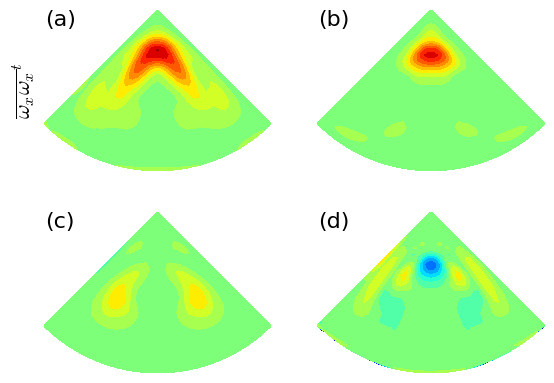
\includegraphics[width=0.6\linewidth]{ub_ox1gen_map.png}}
\caption{Для решения с верхней ветви в сечении, где амплитуда пульсаций достигает наибольшей величины, представлена величина $\overline{\omega'_x \omega'_x}^t$ (график a) и вклад в её формирование со стороны слагаемых \eqref{time_ox1gen_terms1} (график b),  слагаемых  \eqref{time_ox1gen_term2} (график с) и других слагаемых в правой части уравнения \eqref{time_ox1_eq} (график d). }
\label{ub_ox1gen_pic}
\end{figure}
\end{comment}

\section{Исследование решений в виде бегущей волны в течении в круглой трубе}

\section{Исследование решений в виде бегущей волны в плоском течении Пуазейля}

Кроме движения жидкости в круглой трубе в работе также было исследованы некоторые случаи движения жидкости в плоском канале Пуазейля. Постановка задачи в этом случае близка к постановке в круглой трубе. В области течения вводится ортогональная системы координат $(x,y,z)$. Ось $x$ направлена вдоль потока, ось $y$ --- по нормали к стенке, ось $z$ --- в трансверсальном направлении. Движение жидкости полагается удовлетворяющем уравнениям Навье-Стокса \eqref{NSeq_Re} и условию несжимаемости \eqref{eq0_Re}. На твердой стенке, расположенной при $y = 0$, ставятся условия прилипания:
\begin{equation}
\v = 0 \text{, при } y = 0
\end{equation}
При $y = 1$ ставится условие проскальзывания, аналогичное условию на оси трубы при дополнительных условиях симметрии в угловом направлении \eqref{sym_eq} и \eqref{per_eq}. Условие проскальзывания имеет вид:
\begin{equation}
\pd{u}{y} = v = \pd{w}{y} = \pd{p}{y} = 0 \text{, при } y = 1
\end{equation}
Здесь $(u,v,w)$ --- компоненты вектора скорости в декартовой системе координат. В качестве единицы длины, таким образом, выступает полуширина канала. Вдоль потока и в трансверсальном направлении ставятся условия периодичности с периодом $L_x$ и $L_z$ соответственно:
\begin{equation}\label{duct_xper_eq}
(\v,p)(x,y,z) = (\v,p)(x+L_x,y,z)
\end{equation}
\begin{equation}\label{duct_zper_eq}
(\v,p)(x,y,z) = (\v,p)(x,y,z+L_z)
\end{equation}
Также, по аналогии с постановкой задачи в трубе, в трансверсальном направлении ставится условие отражения относительно плоскости $z = 0$:
\begin{equation}\label{duct_sym_eq}
(u,v,w,p)(x,y,z) = (u,v,-w,p)(x,y,-z)
\end{equation}
Условия \eqref{duct_zper_eq} и \eqref{duct_sym_eq} могут быть заменены условиями проскальзывания при $z = 0$ и $z = L_z/2$, имеющим вид:
\begin{equation}
\pd{u}{z} = \pd{v}{z} = w = \pd{p}{z} = 0 \text{, при } z = 0, L_z/2 
\end{equation}
Таким образом, расчетная область представляет собой параллелепипед размера $L_x \times 1 \times L_z/2$. Жидкость приводится в движение внешним перепадом давления, определяемым из условия постоянства удельного расхода. В качестве единицы скорости выступает наибольшая скорость в течении Пуазейля. Условие постоянства удельного расхода в безразмерном виде имеет в этом случае вид:
\begin{equation}
\frac{1}{S}\int_{S} u\,dy\,dz = 2/3
\end{equation}
Здесь $S$ --- поперечное сечение трубы и его площадь. Задача поставлена. 


\begin{figure}
\center{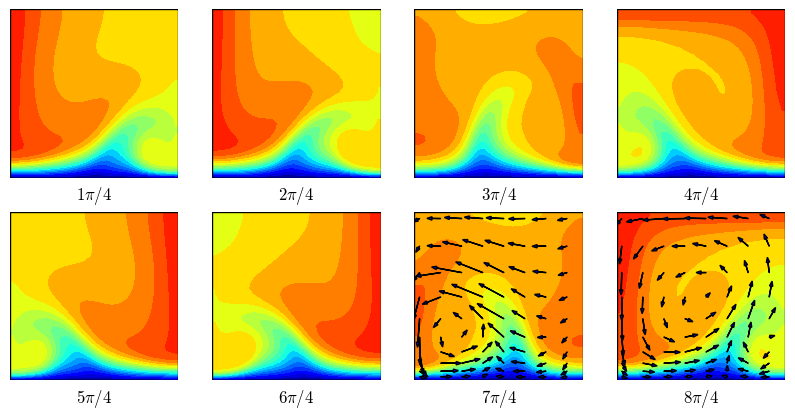
\includegraphics[width=1\linewidth]{duct_turb_map.png}}
\caption{Поле скорости бегущей волны, выделенной из турбулентного течения в плоском канале. Приведена продольная скорости в поперечном сечении в различные фазы течения. На последних двух изображениях приведена также поперечная компонента движения. Твердая стенка находится внизу.} 
\label{duct_turb_tw_pic}
\end{figure}

Было обнаружено, что в расчетной области небольшого размера при небольших значениях числа Рейнольдса турбулентное движение напоминает некоторую бегущую волну. Турбулентное поле скорости оказалось удачным начальным приближением для точной бегущей волны, с которым метод Ньютона сходится. Бегущую волну можно рассматривать, как частный случай условно периодического по времени решения. Для её нахождения может быть использован код, написанный для поиска периодических решений. Параметр $T$, выступающий в качестве периода решения по времени, в данном случае выступает в качестве параметра расчета, не влияющего на результат. Однако отметим, что увеличения значения $T$ позволяет существенным образом сократить число итераций метода решения линейной системы, выполняемого на каждом шаге метода Ньютона. 


\begin{figure}
\center{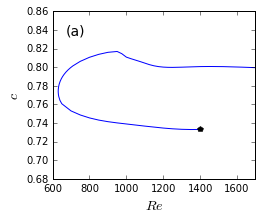
\includegraphics[width=0.45\linewidth]{duct_turb_tw_cf.png}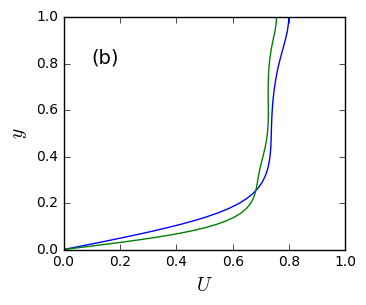
\includegraphics[width=0.45\linewidth]{duct_turb_tw_umean.png}}
\caption{(a) --- зависимость фазовой скорости волны $c$ от числа Рейнольдса $\Re$, черной точкой обозначено исходное решение, принадлежащее верхней ветви; (b) --- средний профиль скорости решения типа бегущей волны с нижней и верхней ветвей, $\Re = 1400$.} 
\label{duct_turb_tw_contin}
\end{figure}


Бегущая волна из турбулентного течения выделена при $L_x = 5$, $L_z = 2$, $\Re = 1400$. Её фазовая скорости равна $c_{tw} = 0.73$. Расчетная сетка, на которой было найдено решение, содержит $64 \times 40 \times 32$ ячеек. Форму бегущей волны позволяет представить рисунок \ref{duct_turb_tw_pic}. На нем изображена продольная скорость в нескольких сечениях трубы, покрывающих один период изменения решения в пространстве (а также во времени). В центре расчетной области около стенки можно выделить полосу замедления, смещающуюся периодическим образом в направлении $z$. Она возникает за счет действия вихрей, расположенных по бокам от полосы замедления в шахматном порядке. Для того, чтобы продемонстрировать существование вихрей, на рисунке \ref{duct_turb_tw_pic} в двух сечения представлена также поперечная компонента скорости. Хотя основные элементы цикла самоподдержания в бегущей волне присутствуют, повторить рассуждения, разработанные при исследовании модельного порыва, для этого решения в полной мере не удается. Амплитуда смещения полосы замедления оказывается слишком велика, так что стандартный метод разделения поля скорости на среднюю и пульсационную составляющие не дает ожидаемого результата. Среднее течение, полученное таким образом, не адекватно воспроизводит форму полос. Метод продления решения по параметру позволяет перевести выделенную бегущую волну к тем значениям параметров, при которых стандартный метод разделения на среднюю и пульсационную составляющие движения дает ожидаемый результат. 




Продлевая выделенную бегущую волну в сторону снижения числа Рейнольдса, удалось достичь точки бифуркации при $\Re = 630$, в которой рождается две ветви решения, и перейти с верхней ветви решения на нижнюю. Зависимость фазовой скорости волны $c_{tw}$ от числа Рейнольдса $\Re$ приведена на рисунке \ref{duct_turb_tw_contin}(a). Для нижней ветви характерны меньшая амплитуда пульсаций, большая фазовая скорость, однако структура решения сохраняется. На рисунке \ref{duct_turb_tw_contin}(b) приведен средний профиль скорости для исходного решения и решения с нижней ветви при том же числе Рейнольдса $\Re = 1400$. Профиль скорости наполненный, на нижней и верхней ветви отличается мало и напоминает профиль скорости в турбулентном потоке. Для дальнейшего анализа выбрано решение, для которого также $\Re = 1400$, $c_{tw} = 0.8$. 

\begin{figure}
\center{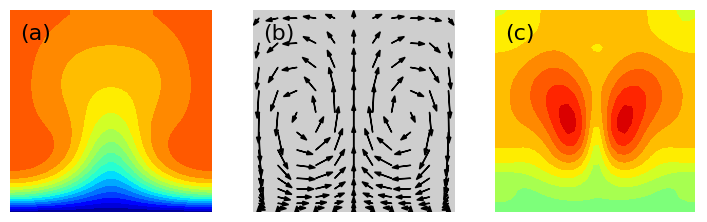
\includegraphics[width=0.9\linewidth]{duct_turb_low_tw_map.png}}
\caption{Нижняя ветвь решения типа бегущей волны, $\Re = 1400$. Приведены: (a) --- средняя продольная компонента скорости $U$, (b) --- средняя поперечная компонента скорости $(V,W)$, (c) --- амплитуда пульсаций $\v_n$.} 
\label{duct_turb_tw_pic}
\end{figure}

Поле скорости $\v$ решения с нижней ветви разделяется на среднюю $\V = \overline{\v}^x$ и пульсационную $\v_n = \v - \V$ составляющие осреднением вдоль трубы. В этом случае среднее поле скорости воспроизводит полосы пониженной и повышенной скорости. Продольная компонента среднего поля скорости $U$ изображена на рисунке \ref{duct_turb_tw_pic}(a). Полоса замедления проходит через центр расчетной области вблизи стенки. Полосы ускорения расположены на границах расчетной области при $z = 0$ и $z = 1$. Полосы возникают с результате действия продольных вихрей. На рисунке \ref{duct_turb_tw_pic}(b) представлена поперечная компонента скорости среднего течения $(V,W)$. Поперечное движение может быть ассоциировано с парой продольных вихрей, расположенных по бокам от полосы замедления. Пульсационная составляющая движения возникает в результате периодического смещения полосы замедления в угловом направлении. Амплитуда пульсаций приведена на рисунке \ref{duct_turb_tw_pic}(c). Они сосредоточены в областях между полосами пониженной и повышенной скорости. Как и в других случаях, пульсационная составляющая движения в этом случае возникает в результате линейной неустойчивости среднего течения. Можно отметить, что и в этом случае поле скорости $(U,0,0)$ оказывается линейно устойчиво, так что пренебрежение поперечным движением качественно меняет характеристики устойчивости среднего течения. 

\begin{figure}
\center{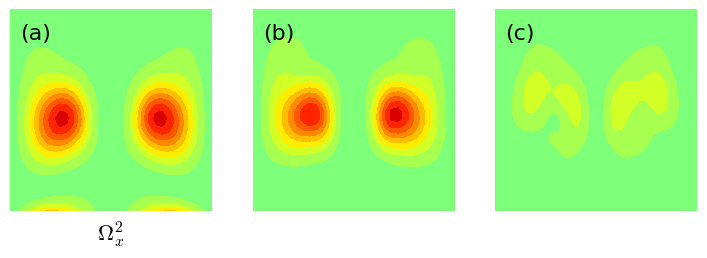
\includegraphics[width=0.9\linewidth]{duct_turb_tw_OXgen.png}}
\caption{Механизм генерации $\Omega_x$ для бегущей волны в плоском канале. Приведено значение $\Omega_x^2$ (a) и вклад в его образование со стороны слагаемых \eqref{OXgen_terms} (b) и суммы других слагаемых в правой части уравнения \eqref{OX_eq} (c).} 
\label{duct_turb_tw_OXgen_pic}
\end{figure}

Выделенное решение позволяет наиболее ярко продемонстрировать механизм образования продольной завихренности. Продольным вихрям соответствуют области повышенной амплитуды стационарной продольной завихренности $\Omega_x$. Квадрат стационарной продольной завихренности изображен на рисунке \ref{duct_turb_tw_OXgen_pic}(a). Форму поля продольной завихренности определяет слагаемое \eqref{OXgen_terms}. Его вклад в $\Omega_x^2$ приведен на рисунке \ref{duct_turb_tw_OXgen_pic}(b). Вклад других слагаемых в правой части уравнения \eqref{OX_eq} представлен на рисунке \ref{duct_turb_tw_OXgen_pic}(с). Их суммарное влияние незначительно, хотя оказывается положительным. Таким образом, нет сомнения, что за образование продольных вихрей ответственны слагаемые \eqref{OXgen_terms}, как и в предыдущих случаях. 

\begin{figure}
\center{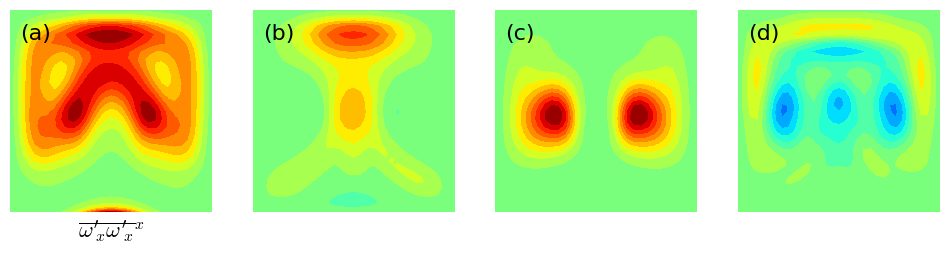
\includegraphics[width=1\linewidth]{duct_turb_tw_ox1gen.png}}
\caption{Механизм генерации $\omega_x'$ для бегущей волны в плоском канале. Приведено значение $\overline{\omega'_x \omega'_x}^x$ (a) и вклад в его образование со стороны слагаемых \eqref{ox1gen_add_terms} (b), \eqref{ox1gen_main_terms} (c) и других слагаемых в правой части уравнения \eqref{ox1_eq} (d).}
\label{duct_turb_tw_ox1gen_pic}
\end{figure}

Образование пульсаций продольной завихренности $\omega'_x$ также происходит в соответствии с выделенным в работе механизмом. Средний вдоль трубы квадрат $\omega'_x$ приведен на рисунке \ref{duct_turb_tw_ox1gen_pic}(a). Как и в предыдущих случаях, на месте продольных вихрей определяющий вклад дает слагаемое \eqref{ox1gen_main_terms}. Его вклад в $\overline{\omega'_x \omega'_x}$ изображен на рисунке  \ref{duct_turb_tw_ox1gen_pic}(c). На рисунке \ref{duct_turb_tw_ox1gen_pic}(b) приведен вклад слагаемого \eqref{ox1gen_add_terms}, связанного с наклоном нормальных к стенке вихрей, возникающих в пульсационной составляющей движения. В отличии от случае модельного порыва, в этом случае на месте продольных вихрей вклад этого слагаемого пренебрежимо мал, что гарантирует, что оно не участвует в образовании продольных вихрей. Вклад других слагаемых, приведенных на рисунке \ref{duct_turb_tw_ox1gen_pic}(с) оказыватеся отрицательным на месте продольных вихрей. Это вновь может говорить о неточности при разделении слагаемых уравнения \eqref{ox1_eq} на связанные и несвязанные с образование продольной завихренности группы.


%\section{Исследование решения в виде бегущей волны в плоском канале}

В плоском канале может быть найдено решение на сепаратрисе. Метод поиска решения на сепаратрисе в непротяженной расчетной области в постановке, приведенной в предыдущем разделе, позволяет получить бегущую волну, представляющую еще одно семейство решений. Расчеты были выполнены при $L_x = 5$, $L_z = 2.4$, $\Re = 2000$. Возникающая на сепаратрисе бегущая волна в этом случае имеет фазовую скорость $c_{tw} = 0.97$, что близко к максимальной скорости в потоке. Средний профиль её скорости мало отличается от профиля ламинарного течения. Интенсивность пульсаций и движения в поперечной плоскости в этом случае на порядок ниже, чем в бегущей волне, выделенной из турбулентного течения. Тем не менее, структура течения оказывается такой же, как и в других исследованных течениях. В потоке может быть выделена полоса замедления, проходящая через центра расчетной области. Продольная компонента среднего поля скорости $U$ приведена на рисунке \ref{duct_edge_tw_means_pic}(a). В этом случае полоса замедления, как и другие особенности решения, оказывается значительно удалена от твердой стенки. За образование полосы замедления ответственно вторичное течение. Поперечная компонента среднего течения приведена на рисунке \ref{duct_edge_tw_means_pic}(b). Она соответствует паре продольных вихрей, расположенных по бокам от полосы замедления, поддерживающих её существование. Пульсационная составляющая движения сосредоточена в центре канала, и соответствует периодическому смещению области замедления в направлении $z$. Амплитуда пульсаций представлена на рисунке \ref{duct_edge_tw_means_pic}(с). Как и в предыдущих случаях, пульсационная составляющая движения возникает вследствие линейной неустойчивости среднего течения. Кроме того, учет поперечных компонент среднего течения при исследовании его на устойчивость необходим, так как поле скорости $(U,0,0)$ линейной устойчиво. 


\begin{figure}
\center{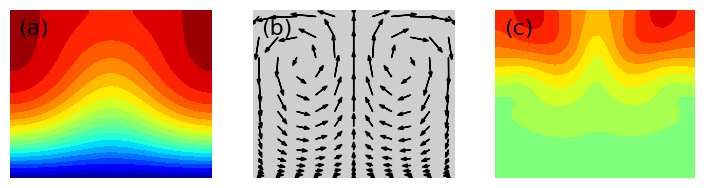
\includegraphics[width=0.9\linewidth]{duct_edge_tw_means.png}}
\caption{Бегущая волна, возникающая на сепаратрисе в плоском канале, $\Re = 2000$. Приведена стационарная продольная составляющая скорости $U$ (a), стационарная поперечная составляющая скорости $(V,W)$ (b) и амплитуда пульсаций $\v_n$ (с).} 
\label{duct_edge_tw_means_pic}
\end{figure}

Механизм образования продольных вихрей в этом случае также согласуется с уже существующими представлениями. Продольные вихри соответствуют областям повышенной концентрации продольной завихренности $\Omega_x$. Квадрат стационарной продольной завихренности $\Omega_x^2$ изображен на рисунке \ref{duct_edge_tw_OXgen_pic}(a). Нет сомнений, что за образование стационарных продольных вихрей ответственны слагаемые \eqref{OXgen_terms}. Их вклад в формирование $\Omega_x^2$ представлен на рисунке \ref{duct_edge_tw_OXgen_pic}(b). Он значительно превосходит по величине вклад других слагаемых, приведенный на рисунке \ref{duct_edge_tw_OXgen_pic}(c), и определяет форму поля $\Omega_x^2$. Механизм образования пульсаций продольной завихренности $\omega'_x$ в этом случае также согласуется с уже разобранными случаями. 

\begin{figure}
\center{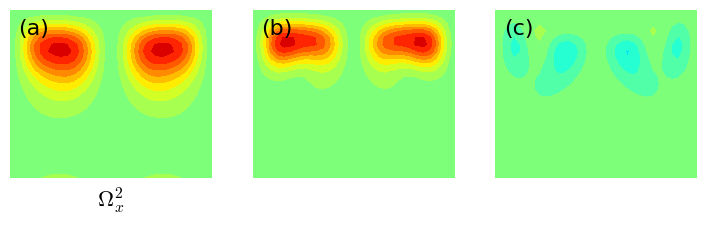
\includegraphics[width=0.9\linewidth]{duct_edge_tw_OXgen.png}}
\caption{Механизм генерации продольных вихрей в бегущей волне, возникающей на сепаратрисе. Приведено значение $\Omega_x^2$ (a) и вклада в его образование со стороны слагаемых \eqref{OXgen_terms} (b) и суммы других слагаемых в правой части уравнения \eqref{OX_eq} (c).}
\label{duct_edge_tw_OXgen_pic}
\end{figure}


\section{Выводы по главе}

В работе, кроме модельного порыва, были найдены и другие инвариантные решения, также допускающие строгое исследование. Их анализ в некоторой степени позволяет установить общность полученных при исследовании модельного порыва результатов. Для всех исследованных решений основные элементы цикла самоподдержания сохраняются, что говорит об их универсальности и позволяет надеяться, что в некотором виде они могут быть найдены в пристенном турбулентном течении непосредственно. 

Продлевая модельный порыв по числу Рейнольдса удалось получить новое условно периодическое локализованное в пространстве решение. Его характеристики оказываются ближе к характеристикам турбулентного порыва, и мы полагаем, что полученные при его исследовании результаты имеют большее отношение к турбулентности. Его анализ показал, что все особенности движения, выделенные при изучении модельного порыва, в полной мере справедливы для найденного решения. Так как оба решения являются представителями одного семейства, можно ожидать, что они воспроизводят общий физический механизм самоподдержания. Тем не менее, полученный результат говорит о том, что механизм самоподдержания сформулирован нами в подходящих терминах; выделенные особенности движения связаны с механизмом самоподдержания существенным образом. 

Также, в плоском канале удалось выделить бегущую волну непосредственно из турбулентного течения. Можно ожидать, что найденное решение воспроизводит особенности, характерные для пристенной турбулентности, хотя её динамика была значительным образом редуцирована наложением условий периодичности в продольном и трансверсальном направлениях. Это может привести к формированию в течении структур, не характерных для свободного турбулентного течения. Важно, что кроме дополнительных условий периодичности, других условий, навязывающих структуру течению, нет. В потоке естественным образом формируется полоса пониженной скорости, расположенная вблизи стенки трубы. Она подвержена значительным по амплитуде колебаниям, что не позволяет, применяя стандартный метод, разделить поле скорости на среднюю и пульсационную части. Однако выделенное решение продлением по числу Рейнольдса было приведено к параметрам, при которых амплитуда пульсаций снижается до уровня, при котором стандартный метод разделения дает желаемый результат. Для полученного таким образом решения справедливы все особенности движения, связанные с числом самоподдержания, выделенные в работе.

Также в плоском канале было была получена бегущая волна, принадлежащая сепаратрисе. Для неё характерна низкая амплитуда вторичного течения и пульсаций, её среднее поле скорости существенно отличается от поля скорости бегущей волны, выделенной в турбулентном течении, однако и в этом решении основные особенности движения, связанные с циклом самоподдержания, выделены. Кроме представленных в главе решений, в работе были получены некоторые другие инвариантные решения. В частности, удалось выделить бегущую волну из турбулентного течения в круглой трубы. Оказалось, что выделенная бегущая волна принадлежит тому же семейству, которому принадлежит бегущая волна, возникающая на сепаратрисе, но если вторя принадлежит нижней ветви, то первая -- верхней. Бегущая волна с верхней ветви повторяет форму бегущей волны, возникающую внутри модельного порыва на верхней ветви. В силу свой избыточности, результаты для неё в главе не приведены. 

Можно отметить, что в ряде случаев есть основания полагать, что слагаемые, отвечающие за формирование продольных вихрей, выделены не точно. Вероятно, уточнить их позволит развитие представлений о физическом механизме, ответственном за этот процесс. Кроме того, метод разделения на среднюю и пульсационную составляющие течения оказался не эффективным при исследовании бегущей волны, выделенной из турбулентного течения. Вероятно, аналогичные сложности могут возникнуть при изучении турбулентного течения непосредственно. Для преодоления возникшего затруднения необходимо разработать новый метод разделения течения на компоненты, пригодный для потоков с большой амплитудой пульсаций.

То обстоятельство, что выделенный при изучении течения в трубе механизм самоподдержания справедлив также и для течений в плоском канале говорит о том, что он связан с кривизной стенки существенным образом. 

Отметим также, что все исследованные решения найдены при условии отражения в трансверсальном направлении. Существует вероятность, что такое условие навязывает некоторую структур течению, не характерную для свободных потоках. 






